\documentclass[ALICE,manyauthors]{ALICE_analysis_notes}
%\documentclass[ALICE,manyauthors]{ALICE_scientific_notes}
%
%\newcommand{\jpsi}{\rm J/$\psi$}
%\newcommand{\psip}{$\psi^\prime$}
%\newcommand{\jpsiDY}{\rm J/$\psi$\,/\,DY}
%\newcommand{\dd}{\mathrm{d}}
%\newcommand{\chic}{$\chi_{\rm c}$}
%\newcommand{\ezdc}{$E_{\rm ZDC}$}
%\newcommand{\red}{\textcolor{red}}
%\newcommand{\blue}{\textcolor{blue}}
\newcommand{\slfrac}[2]{\left.#1\right/#2}
\usepackage{rotating}
%
\begin{document}%
%%%%%%%%%%%%% ptdr definitions %%%%%%%%%%%%%%%%%%%%%
%
%%%%%%%%%%%%%%%  Title page %%%%%%%%%%%%%%%%%%%%%%%%
%
\begin{titlepage}
%
\PHnumber{ALICE-ANA-2014-xxx} 
\PHdate{\today}
%
%%% Put your own title + short title here:
\title{Analysis of light vector mesons in p--p collisions at $\sqrt{s}=$ 13 TeV}
\ShortTitle{Analysis of Light Vector Mesons}   % appears on right page headers
%
\author{Jonathan Kley$^{1}$}
\author{
1. Technical University of Munich\\
}
\author{Email: jonathan.kley@cern.ch}
%
\ShortAuthor{ALICE Analysis Note 2012}      % appears on left page headers, do not change
%
\begin{abstract}
Here goes your abstract
\end{abstract}
\end{titlepage}
\tableofcontents
\newpage

\section{Introduction\footnote{The introduction is mostly based on \cite{ChiSym} with other references used where cited.}}
\label{sec:Introduction}
With the exploration of the phase diagram of nuclear matter has come the idea of the Quark gluon plasma (QGP), a state of matter where confinement is abolished and quarks and gluons can move quasi-freely. However, they still interact strongly, so the medium behaves more like a perfect liquid than a gas. The QGP is created when a critical temperature of $T_c = (154 \pm 9)$ MeV is exceeded \cite{tcrit}. In the laboratory heavy ion collisions are used to deposit a lot of energy in a small spatial volume making it possible to exceed the critical temperature and creating a QGP. After thorough theoretical investigations, experiments in the late 80s started looking for the QGP, but definite traces where only found in the early 2000s by the RHIC experiments at Brookhaven National Laboratory \cite{QGPrhic}. Since then other experiments also joined in on the search for the QGP. After the SPS experiments at CERN could not find any traces of the formation of a QGP, CERN built a dedicated LHC experiment to investigate heavy ion collisions and the QGP, the ALICE experiment \cite{ALICEproposal} which was also used to obtain the data which is analysed here. \\
Because of the short life time (of $O(10 \frac{fm}{c})$ \cite{QGPlifetime}) of the QGP and its strongly interacting nature, it is very difficult to gain information about the properties of the QGP. This is mainly because particles either live too long to decay inside the QGP and therefore lose their information. Or if they decay inside the QGP, their decay products might interact strongly and lose the information they carry about the QGP through scattering in the QGP. So, the most important probes to investigate the QGP are short-lived particles which decay into particles which only interact electromagnetically. One candidate are vector mesons which carry the same quantum numbers as photons ($J^P = 1^{-}$) and couple to them (and therefore effectively to dileptons) as explained by the vector-dominance model. The dileptons are a very clean experimental probe and can be identified with high precision in the ALICE TPC. \\
One of the most interesting aspects of the QGP is the possible restoration of the chiral symmetry which might also be connected to a phase transition in the phase diagram of nuclear matter. There are many implications of this possible restoration of chiral symmetry on the particle spectrum of QCD which in reverse can also be used to check if our fundamental theory of the strong interaction - QCD - is correct. One system which should in theory be affected by the restoration of chiral symmetry and also  is the $\rho$-$a_1$ system. If chiral symmetry is present these two particles are related to each other which has consequences on their so-called spectral functions. \\
This work is a feasibility study of the measurement of the $a_1$ meson at the ALICE experiment in pp collisions. Along the $a_1$ meson we also try to identify vector mesons which appear in the same decay channels to double check our results. \\
This paper is structured as follows. In section \ref{sec:Introduction} I will discuss the chiral symmetry of QCD and its consequences in more detail, also including implications on the $\rho$-$a_1$ system. I will then discuss the details of the data analysis in section \ref{sec:Analysis} including the analysis strategy and particle cuts and event selection. Finally in section \ref{sec:Results}, I will discuss the results and give a quick outlook in section \ref{sec:Outlook}.

\subsection{The QCD Lagrangian}
To understand the effects of the strong interaction we use the theory which has been proven most successful in this matter in the end of the last century: QCD. We start from the classic Lagrangian of QCD with 3 flavours which is the unique Lagrangian which is invariant under a gauged SU(3) symmetry
\begin{equation}
\label{eqn:LQCD}
\Lag_{QCD} = \bar{\psi}_i \left( i\gamma_{\mu} D^{\mu} - m \right)_{ij} \psi_j - \frac{1}{4} G_{\mu\nu}^a G^{\mu\nu}_a
\end{equation}
where $\psi = \left( u,d,s \right)$ are the quark fields, $D^{\mu} = \partial^{\mu} -igA^{\mu}$ is the covariant derivative in the fundamental representation and $G_{\mu\nu}^a = \partial_{\mu}A_{\nu} - \partial_{\nu}A_{\mu} + g f^{abc} A_{\mu}^b A_{\nu}^c$ is the field strength of the gluon fields $A_{\mu}^a$ with the structure constants $f^{abc}$ of SU(3). \\
Following the usual procedure of perturbative renormalization we can calculate the $\beta$-function in QCD. At 1-loop order it is given by \cite{QCDEllis}
\begin{equation}
\label{eqn:beta}
\beta(\alpha_S) = \mu_R^2 \frac{d\alpha_S}{d\mu_R^2} = - \left( 11 - \frac{2}{3} n_f \right) \frac{\alpha_S^2}{4\pi} + O(\alpha_S^3)  \equiv - \beta_0 \frac{\alpha_S^2}{4\pi} + O(\alpha_S^3)
\end{equation}
where $n_f$ is the number of flavours and $\beta_0$ the 1-loop $\beta$-function coefficient.
Solving the differential equation in eqn. \ref{eqn:beta} in terms of the renormalized scale $\mu_R^2$ we get an expression for the running coupling in QCD. Using the 1-loop expression we get
\begin{equation}
\label{eqn:alpha}
\alpha_S(\mu) = \frac{4\pi}{\beta_0 \log\frac{\mu^2}{\Lambda^2}} 
\end{equation}
where $\Lambda$ is the QCD scale and we fixed $\alpha(\mu) \overset{\mu \rightarrow \Lambda}{\longrightarrow} \infty$. A plot of the running coupling along with the most recent measurements can be seen in fig. \ref{fig:alpha}. \\
From eqn. \ref{eqn:alpha} it is obvious that perturbation theory is not applicable at energy scales close to the fundamental scale of our theory. Unfortunately this is the regime we are interested in, so we have to think of another way to approach scales $\mu < \Lambda_{QCD}$. 
\begin{figure}[t]
	\centering
	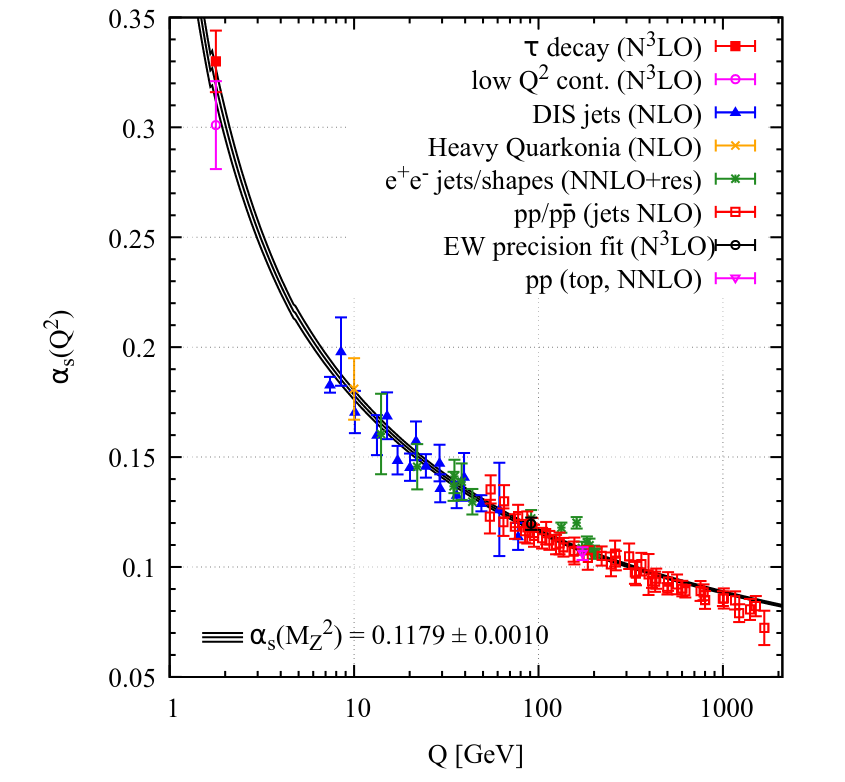
\includegraphics[width=0.55\textwidth]{Figures/alphaQCD}
	\caption{The running coupling of QCD \cite{PDG2018}. Summary of measurements of $\alpha_S$ as a function of the scale $Q$. The order in QCD perturbation theory which was used in the calculation is indicated in brackets.}
	\label{fig:alpha}
\end{figure}
\subsection{Chiral Symmetry of QCD}
One of the ways to approach regimes where $\mu < \Lambda_{QCD}$ is to build an effective Lagrangian based on the symmetries of the fundamental Lagrangian of QCD. In this section we investigate this approach and see which implications it has for the particle spectrum of the theory. \\
We start from the Lagrangian of QCD in eqn. \ref{eqn:LQCD}. Of particular interest to us for the chiral symmetry is the quark term in the Lagrangian which can be split into two parts
\begin{equation}
\Lag_{\mathrm{quarks}} = \bar{\psi} i\gamma_{\mu} D^{\mu} \psi - m \bar{\psi} \psi \equiv \Lag + \delta\Lag
\end{equation}
The suggestive names will make sense in a second. 
Since the doublet of quark fields in $\Lag$ are contracted in an inner product the Lagrangian is invariant under an inner symmetry. In our case this is a U(2) symmetry for both chiralities, so U(2)$_L \times$ U(2)$_R$ in total. We can also think of the symmetries in terms of axial and vector currents instead of left and right handed currents which is more useful in this analysis, so the symmetry group is U(2)$_V \times$ U(2)$_A$. We only consider the SU(2) part of both subgroups, since U(1)$_V$ can be identified with baryon number conservation and U(1)$_A$ is anomalous because th, so it is not a real symmetry of our theory. Let us consider the following SU(2) transformations
\begin{align}
& U_V = \exp \left(-i \alpha^i \frac{\sigma^i}{2} \right) \approx 1 - i\alpha^i \frac{\sigma^i}{2} \in SU(2)_V & \label{eqn:Vtrafo} \\
& U_A = \exp \left(-i \gamma_5 \alpha^i \frac{\sigma^i}{2} \right) \approx 1 - i \gamma_5 \alpha^i \frac{\sigma^i}{2} \in SU(2)_A & \label{eqn:Atrafo}
\end{align}
of the quark fields and their action on $\Lag$
\begin{equation}
\Lag = i \psi^{\dagger} \gamma_0 \gamma^{\mu} D_{\mu} \psi \overset{U_V}{\longrightarrow} i \left( U_V \psi \right)^{\dagger} \gamma_0 \gamma^{\mu} D_{\mu} U_V \psi = i \psi^{\dagger} e^{+i \alpha^i \frac{\sigma^i}{2}} \gamma_0 \gamma^{\mu} D_{\mu} e^{-i \alpha^i \frac{\sigma^i}{2}} \psi = i \bar{\psi} \fsl{D} \psi
\end{equation}
and
\begin{equation}
\Lag = i \psi^{\dagger} \gamma_0 \gamma^{\mu} D_{\mu} \psi \overset{U_A}{\longrightarrow} i \left( U_A \psi \right)^{\dagger} \gamma_0 \gamma^{\mu} D_{\mu} U_A \psi = i \psi^{\dagger} e^{+i \alpha^i \gamma_5 \frac{\sigma^i}{2}} \gamma_0 \gamma^{\mu} D_{\mu} e^{-i \gamma_5 \alpha^i \frac{\sigma^i}{2}} \psi = i \bar{\psi} \fsl{D} \psi
\end{equation}
where we used $\lbr \gamma^{\mu},\gamma_5 \rbr = 0 = \left[ D^{\mu},\gamma_5 \right]$ and $\gamma_5^{\dagger} = \gamma_5$.
So $\Lag$ is invariant under both $U_V$ and $U_A$.
The corresponding currents are
\begin{align}
& j_{\mu}^i = \bar{\psi} \gamma_{\mu} \frac{\sigma^i}{2} \psi & \label{eqn:jV} \\
& j_{5\mu}^i = \bar{\psi} \gamma_{\mu} \gamma_5 \frac{\sigma^i}{2} \label{eqn:jA} \psi & 
\end{align}
Now we can check the effect of the transformations on $\delta \Lag$
\begin{equation}
\delta \Lag = - m \psi^{\dagger}\gamma^0 \psi \overset{U_V}{\longrightarrow} - m \left( U_V \psi \right)^{\dagger}\gamma^0 U_V \psi = - m \psi^{\dagger} e^{+i\alpha^i \frac{\sigma^i}{2}} \gamma^0 e^{-i\alpha^i \frac{\sigma^i}{2}} \psi = - m \bar{\psi} \psi
\end{equation}
and 
\begin{equation}
\delta \Lag = - m \psi^{\dagger}\gamma^0 \psi \overset{U_A}{\longrightarrow} - m \left( U_A \psi \right)^{\dagger}\gamma^0 U_A \psi = - m \psi^{\dagger} e^{+i \gamma_5 \alpha^i  \frac{\sigma^i}{2}} \gamma^0 e^{-i \gamma_5 \alpha^i \frac{\sigma^i}{2}} \psi = - m e^{2i \gamma_5 \alpha^i \frac{\sigma^i}{2}} \bar{\psi} \psi \neq \delta \Lag
\end{equation}
where we used the same identities as above. We see that the mass term is not invariant under axial transformations while it is left invariant by vector transformations. The axial symmetry is therefore explicitly broken by the quark mass term. But as long as the quark masses are smaller than the scale of our theory we can still use the symmetry as an approximate symmetry. This is indeed the case, since $m_u,m_d \sim O(5 \ \mathrm{MeV}) \ll \Lambda_{QCD} \simeq 200 \ \mathrm{MeV}$.

\subsection{Spontaneous Chiral Symmetry Breaking}
With our 2 quark fields we can now build bosonic fields that have the quantum numbers of the mesons in nature. We find
\begin{align*}
& \mathrm{pion-like \ state:} \ \vec{\pi} \equiv i \bar{\psi} \vec{\sigma}\gamma_5 \psi; \qquad \mathrm{sigma-like \ state:} \ \sigma \equiv \bar{\psi}\psi & \\
&\mathrm{rho-like \ state:} \ \vec{\rho}_{\mu} \equiv \bar{\psi} \vec{\sigma}\gamma_{\mu} \psi; \qquad a_1\mathrm{-like \ state:} \ \vec{a}_{1 \mu} \equiv \bar{\psi} \vec{\sigma}\gamma_{\mu}\gamma_5 \psi &
\end{align*}
Of particular interest to us will be the $\rho$ and the $a_1$ states because they correspond to the conserved currents from eqn. \ref{eqn:jV} and \ref{eqn:jA} and therefore seem to be closely related to the chiral symmetry. Let us see now how these particles transform under the chiral transformations in infinitesimal form, so we can understand the symmetry better.
Starting with the $\pi$ state and with the vector transformation from eqn. \ref{eqn:Vtrafo} we get
\begin{align*}
i \bar{\psi} \sigma^i \gamma_5 \psi & \overset{U_V}{\longrightarrow} i \left( U_V \psi \right)^{\dagger} \gamma^0 \sigma^i\gamma_5 U_V \psi = i \bar{\psi} \sigma^i\gamma_5 \psi + \alpha^j \left( \bar{\psi} \sigma^i \frac{\sigma^j}{2} \gamma_5 \psi - \bar{\psi} \frac{\sigma^j}{2} \sigma^i \gamma_5 \psi \right) + O(\alpha^2) = & \\
& = i \bar{\psi} \sigma^i\gamma_5 \psi + i \alpha^j \epsilon^{ijk} \bar{\psi} \sigma^k\gamma_5 \psi & \numberthis
\end{align*}
where we have used the $SU(2)$ algebra $\left[\sigma^i,\sigma^j \right] = 2i \epsilon^{ijk} \sigma^k$. We can do similar calculations for all of the other states as well and get for the vector transformations
\begin{align}
\vec{\pi} \overset{U_V}{\longrightarrow} & \vec{\pi} + \vec{\alpha} \times \vec{\pi} & \\
\sigma \overset{U_V}{\longrightarrow} & \sigma & \\
\vec{\rho}_{\mu} \overset{U_V}{\longrightarrow} & \vec{\rho}_{\mu} + \vec{\alpha} \times \vec{\rho}_{\mu} & \\
\vec{a}_{1 \mu} \overset{U_V}{\longrightarrow} & \vec{a}_{1 \mu} + \vec{\alpha} \times \vec{a}_{1 \mu}
\end{align}
Which is also what we expect when we identify $SU(2)_V$ with isospin. $\vec{\pi}$, $\vec{\rho}_{\mu}$ and $\vec{a}_{1 \mu}$ are all in the fundamental representation of isospin and are therefore changed by an isospin rotation. Whereas, $\sigma$ is a scalar under isospin and is therefore not affected. \\
However, under the axial transformations the particles mix as follows
\begin{align}
\vec{\pi} \overset{U_A}{\longrightarrow} & \vec{\pi} + \vec{\alpha} \sigma & \\
\sigma \overset{U_A}{\longrightarrow} & \sigma - \vec{\alpha} \cdot \vec{\pi} & \\
\vec{\rho}_{\mu} \overset{U_A}{\longrightarrow} & \vec{\rho}_{\mu} + \vec{\alpha} \times \vec{a}_{1 \mu} & \\
\vec{a}_{1 \mu} \overset{U_A}{\longrightarrow} & \vec{a}_{1 \mu} - \vec{\alpha} \times \vec{\rho}_{\mu}
\end{align}
Since 2 pairs of particles are rotated into each other by axial rotations, this suggests that these particles have the \textit{same} mass or after the explicit breaking of $SU(2)_A$ by the quark mass term at least a \textit{similar} mass. But this does not seem to be the case in nature, since e.g. the $a_1$ has a mass of $m_{a_1} \simeq 1260$ MeV which is almost double the mass of the $\rho$ meson with a mass of $m_{\rho} \simeq 770$ MeV. \\
So, clearly $m_{a_1} \not\simeq m_{\rho}$ and $SU(2)_A$ can not be a symmetry of the vacuum and must therefore be spontaneously broken: $SU(2)_V \times SU(2)_A \rightarrow SU(2)_V$. This can also be seen from the vacuum expectation value (VEV) of the term $\bar{\psi}\psi$ 
\begin{equation}
\label{eqn:vev} 
\langle 0 | \bar{\psi} \psi | 0 \rangle \overset{U_A}{\longrightarrow} \langle 0 |   \bar{\psi} e^{-2i \gamma_5 \alpha^i \frac{\sigma^i}{2}} \psi | 0 \rangle
\end{equation}
which would be invariant if the vacuum was invariant: $U_A | 0 \rangle = e^{-i \gamma_5 \alpha^i \frac{\sigma^i}{2}} | 0 \rangle = | 0 \rangle$. However, this is not the case in nature as we just discussed. Therefore, $SU(2)_A$ must be spontaneously broken and $\bar{\psi}\psi$ - the so-called chiral condensate - must develop a vacuum expectation value $\langle \bar{\psi}\psi \rangle = - \left( 250 \text{MeV} \right)^3$. We can use the VEV as an order parameter for the breaking of $SU(2)_A$. If the symmetry is not broken the VEV is zero and if we have a finite VEV the symmetry is broken as we expect from an order parameter. \\
We can now interpret the three spin-0 particles $\vec{\pi}$ from above as the Goldstone bosons of the spontaneously broken $SU(2)_A$. If $U(1)_A$ wasn't anomalous, we could identify the $\sigma$ as its Goldstone boson, which in the case of three flavours can be identified with the $\eta'$. \\
We could now turn on the usual machinery for spontaneously broken symmetries and construct the effective Lagrangian of the pions. But since we don't do any original calculations in this paper, let us skip that and look at some implications of the spontaneous symmetry breaking and the possible return of the symmetry. Especially in the for the vector mesons whose field configurations correspond to the conserved currents.

\subsection{Effects of Hot and Dense Matter on Chiral Symmetry}
In this section I want to discuss the possible effects of hot and dense matter - like a QGP - on observables. In our case only the temperature dependence is interesting, since the ALICE experiment operates at zero baryon chemical potential. The QGP in ALICE is created by depositing as much energy as possible in a small spatial volume and then hoping to reach a temperature $T > T_c$. \\
Let us start with the discussion of the order parameter of chiral symmetry which we just defined in eqn. \ref{eqn:vev}. Gerber and Leutwyler showed that up to 3-loop order the temperature dependence of $\langle \bar{\psi} \psi \rangle$ for $T < T_c$ and massless quarks is given by \cite{OrdPar3loop}
\begin{equation}
\frac{\langle \bar{\psi} \psi \rangle(T)}{\langle \bar{\psi} \psi \rangle(T=0)} = 1 - x - \frac{1}{6} x^2 - \frac{16}{9} x^3 \ln \frac{T}{\Lambda_q}
\end{equation}
where $x = \frac{T^2}{8f^2}$, the relevant temperature scale is $\sqrt{8}f \simeq 250$ MeV with $f$ the pion decay constant in the chiral limit and $\Lambda_q = (470 \pm 110)$ MeV. We can see a clear trend of a decreasing order parameter for increasing temperature which suggests a restoration of chiral symmetry if the trend continues. \\
The temperature dependence over a bigger interval can be obtained from lattice QCD. The results of one such calculation can be found in fig. \ref{fig:ordparlat}. Here we can see that the trend indeed continues and chiral symmetry seems to be restored in a QGP.
\begin{figure}[b]
	\centering
	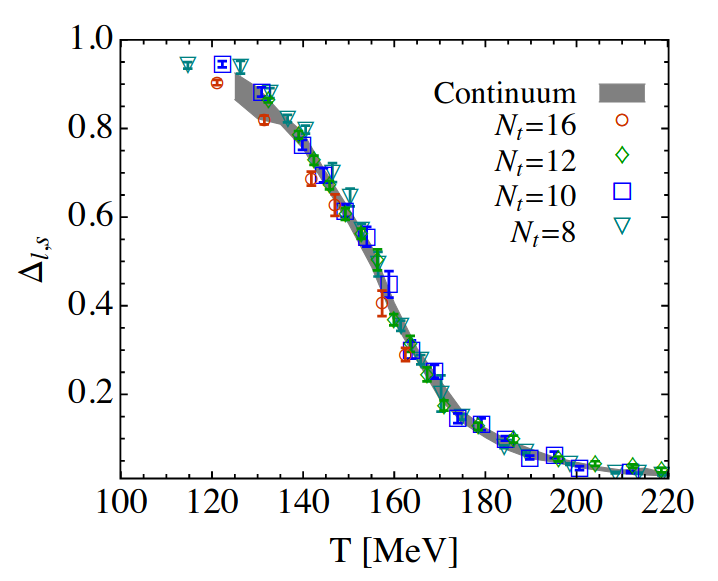
\includegraphics[width=0.45\textwidth]{Figures/ChiralOrderParameterLattice}
	\caption{Lattice calculation of subtracted chiral condensate which is defined as $ \Delta_{l,s} = \frac{\langle \bar{\psi} \psi \rangle_{l,T} - \frac{m_l}{m_s} \langle \bar{\psi} \psi \rangle_{s,T}}{\langle \bar{\psi} \psi \rangle_{l,0} - \frac{m_l}{m_s} \langle \bar{\psi} \psi \rangle_{s,0}}$ with $l = u,d$ \cite{OrdParLat}.}
	\label{fig:ordparlat}
\end{figure}
This of course has consequences on the things we discussed earlier. Let us have a look another look at the axial and vector currents from eqn. \ref{eqn:jV} and \ref{eqn:jA} transforming under the axial transformation
\begin{equation}
\vec{j}^V_{\mu} = \psi^{\dagger} \gamma^0 \gamma_{\mu} \frac{\vec{\sigma}}{2} \psi \overset{U_A}{\longrightarrow} U_A^{\dagger} \bar{\psi} \gamma_{\mu} \frac{\vec{\sigma}}{2} U_A \psi = U_A^{\dagger} \vec{j}^V_{\mu} U_A
\end{equation}
With this transformation rule we can calculate transformation of the correlator
\begin{equation}
\Pi_{\mu\nu} (q) = i \int d^4x e^{iq \cdot x} \langle 0 | \mathcal{T} j^V_{\mu}(x)j^V_{\nu}(0) | 0 \rangle
\end{equation}
in which we can see the vector mesons as resonances. Then assuming chiral symmetry is restored - so $U_A | 0 \rangle = | 0 \rangle$ - we get for the transformation of the correlator
\begin{equation}
\Pi_{\mu\nu}(q) \overset{U_A}{\longrightarrow} i \int d^4x e^{iq \cdot x} \langle 0 | \mathcal{T} U_A^{\dagger} j^V_{\mu}(x) U_A U_A^{\dagger} j^V_{\nu}(0) U_A | 0 \rangle \overset{U_A | 0 \rangle = | 0 \rangle}{=} i \int d^4x e^{iq \cdot x} \langle 0 | \mathcal{T} j^V_{\mu}(x)j^V_{\nu}(0) | 0 \rangle = \Pi_{\mu\nu} (q)
\end{equation}

NOT WHAT WE WANT TO CALCULATE!!! WHAT WE WANT jA = UjV and then <jVjV> = <jAjA> weinberg sumrule Rennecke

"Current correlation functions, QCD sum rules and vector mesons in baryonic matter"



We also see that \cite{ChiPart} correlations function change but might be restored in medium and/or high temperatures. Also from axial trafo of mesons which can be identified with currents
\begin{equation}
j_V \overset{U_A}{\longrightarrow} j_V + \alpha j_A
\end{equation}


show density and temperature dependency of chiral condensate 
might vanish in QGP --> chiral restoration

theory of correlation functions: formula 1 in "Chiral symmetry and mixing of axial and vector correlators in matter" (if chiral symmetry restored we can use jV = UA jA?)



rho has been studied a lot (see below) while there are only few results for a1 (mostly from tau decays)

CERES experiment \cite{CERESrho} and NA60 experiment \cite{NA60rho} reported broadening scenario for $\rho$.



\bibliographystyle{unsrt}  
\bibliography{references}
%
%\input{alice_mynote.tex}               %%%%%%%%%%% put the body of the article here

\end{document}
